\part*{Desarrollo}

% ====================================================== %

\section{Definición del proyecto}

\lipsum[10]

% ====================================================== %

\section{Modelado del Sistema}

% ====================================================== %

\subsection{Traslación del Carro}

Como ya se menciono subsistema de traslación del carro es el encargado de 
mover la carga sobre el puente de la grúa portuaria desde el barco hasta 
el muelle y viceversa en el proceso de carga y descarga de mercancías.

El carro esta simplemente apoyado sobre sus 4 ruedas, no motorizadas, en 
los rieles de la viga principal del puente de la grúa portuaria, 
por lo que se considera que solo puede desplazarse horizontalmente y 
sin resbalamiento.

Su desplazamiento se da por los cables ubicados en sus laterales. Estos
cables trabajan en paralelo y se despliegan en una configuración cerrada
desde el carro hasta el tabor que se encentra en la casa la 
casa de maquinas. El tambor es el elemento que transforma el movimiento
oracional de los motores en movimiento lineal del carro.

Dentro de la casa de maquinas también se encentra el motor que acciona el
carro que esta acoplado con un reductor que a vez esta acoplado con el tambor.
En el eje del motor hay un freno de estacionamiento normalmente cerrado, esto
quiere decir que el freno esta activo cuando no tiene energía y se abre
cuando se energiza.

\subsubsection{Carro}

Se puede considerar al carro como un cuerpo rígido que esta simplemente
apoyado sobre una viga y que tiene la capacidad de desplazare libremente
por esta de forma que desde la perspectiva del marco de referencia se
considere solo un movimiento horizontal. Entonces
el diagrama de fuerzas que actúan sobre el carro es el siguiente:

\begin{figure}[H]
    \centering
    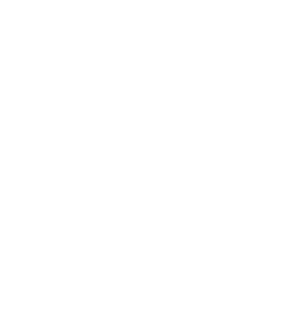
\includegraphics[width=0.5\textwidth]{img/NADA.png}
    \caption{Diagrama de fuerzas del carro}
\end{figure}

La ecuación de movimiento del carro se puede obtener a partir de la segunda
ley de Newton. La ecuación de movimiento es la siguiente:

\begin{equation}
    M_t \ddot{x_t}(t)  = F_{tw}(t) - b_{t} . \dot{x_t}(t) + 2.F_{hw}.sen(\theta(t))
\end{equation}

El diagrama de bloques correspondiente a esta ecuación es el siguiente.

\begin{figure}[H]
    \centering
    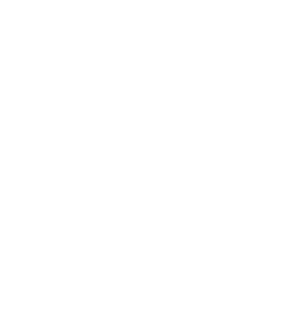
\includegraphics[width=0.5\textwidth]{img/NADA.png}
    \caption{Diagrama de fuerzas del carro}
\end{figure}

\subsubsection{Cable del Carro Elástico Amortiguado}

Los cables conectados al carro, los cuales son los encargados de
transmitir el movimiento generado por el motor, tienen un comportamiento
elástico amortiguado a lo largo de su eje longitudinal. Esto implica que
la longitud de los cables variara según los esfuerzos que se ejerzan
sobre estos.

La siguiente ecuación modela el comportamiento anteriormente dicho.

\begin{equation}
    F_{tw}(t) = K_{tw}.(x_{td}(t) - x_t(t)) + b_{tw}.(\dot{x}_{td}(t) - \dot{x}_t(t))
\end{equation}

Y la siguiente imagen es el modelo que la representa.

\begin{figure}[H]
    \centering
    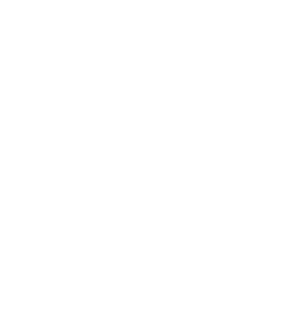
\includegraphics[width=0.5\textwidth]{img/NADA.png}
    \caption{Diagrama de fuerzas del carro}
\end{figure}

\subsubsection{Accionamiento de Traslación del Carro}

Como ya se ha mencionado anteriormente, el accionamiento del carro
se da en la casa de maquinas. Primero, el motor transforma energía 
eléctrica en energía mecánica. Las coordenadas usadas para este se 
corresponden a las del eje rápido. También se recuerda que tiene el
freno asociado a este eje que tiene su modo de funcionamiento. La 
ecuación del motor es: 

\begin{equation}
    J_{tm+tb}.\dot{\omega}_{tm}(t) = T_{tm}(t) + T_{tb}(t, (BBK_t)) - b_{tm}.\omega_{tm}(t) - T_{tml}(t); \text{    } \dot{\theta}_{tm}(t) = \omega_{tm}(t)
\end{equation}

Este freno, normalmente cerrado, mientras este desenergizado un resorte 
estará activo y entregara un torque de frenado. Este torque tiene un 
limite máximo. Cuando se energiza el freno, un mecanismo electro-hidráulico
abre el freno y este deja de actuar.

\begin{equation}
    T_{tb}(t, BBK_t = \text{Off}) = -b_{tb}.\omega_{tm}(t) \text{ , saturado: } -T_{tb MAX} < T_{tb}(t) < T_{tb MAX}\\
\end{equation}

\begin{equation}
    T_{tb}(t, BBK_t = \text{On} ) = 0 \quad \text{N.m}
\end{equation}

Acoplado al motor esta el reductor de engranajes. Se considera que
este tiene un comportamiento rígido y que no tiene backlash. La relación
de transmisión de este esta dada por:

\begin{equation}
    \begin{split}
        \omega_{td}(t). i_t = \omega_{tm}(t)\\
        T_{tml}(t). i_t = T_{td}(t)
    \end{split}
\end{equation}

La ecuación dinámica del tambor, cuyo eje llamamos eje lento, esta dada por:

\begin{equation}
    J_{tm+tb}.\dot{\omega}_{tm}(t) = T_{tm}(t) + T_{tb}(t, (BBK_t)) - b_{tm}.\omega_{tm}(t) - T_{tml}(t);   \dot{\theta}_{tm}(t) = \omega_{tm}
\end{equation}

El tambor cambia el tipo de movimiento de rotacional a traslacional.
Esto se muestra en las siguientes ecuaciones:

\begin{equation}
    v_{td}(t) = r_{td}.\theta_{td}(t); \quad \dot{x}_{td}(t) = v_{td}(t) ; \quad F_{tw}(t).r_{td} = T_{tdl}(t)
\end{equation}

Como se observa en las ecuaciones anteriores, estamos trabajando con 
distintos sistemas de referencia, por lo que es necesario referir el sistema
a un sistema de referencia traslacional del tambor. Para esto en la *ecuación 
del motor* remplazamos con la *ecuación del reductor* y *ecuación* de relación
del tambor despejamos el torque $T_{td}(t)$.

\begin{equation}
    T_{td}(t) = - \frac{J_{tm+tb}. {i_t}^2}{r_{td}}.\ddot{x}_{td}(t) - \frac{b_{tm}. {i_t}^2}{t_{td}}.\dot{x}_{tm}(t) + T_{tm}(t).i_t - T_{tb}(t, (BBK_t)).i_t
\end{equation}

Esta expresión la reemplazamos en la *ecuación* del eje lento y reordenando los 
términos se llega a la siguiente ecuación dinámica que describe el sistema.

\begin{equation}
    J_{eq}. \ddot{x}_{td}(t) = - b_{eq}.\dot{x}_{td}(t) +i_t.(T_{tm}(t) - T_{tb}(t, (BBK_t))) - F_{tw}(t).r_{td}
\end{equation}

Donde:

\begin{equation*}
    \begin{split}
        J_{eq} = \frac{{J_{tm+tb}. {i_t}^2 + J_{td} }}{r_{td}}\\
        b_{eq} = \frac{{b_{tm}. {i_t}^2 + b_{td}}}{r_{td}}
    \end{split}
\end{equation*}

A continuación se muestra el diagrama de bloques que representa el sistema.

\begin{figure}[H]
    \centering
    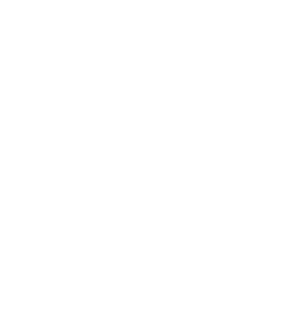
\includegraphics[width=0.5\textwidth]{img/NADA.png}
    \caption{Diagrama de fuerzas del carro}
\end{figure}

% ====================================================== %

\subsection{Izaje de la Carga}

\subsection{Análisis de la Carga}